%!TEX root = ../../csuthesis_main.tex
\chapter{ROV运动控制仿真}
在前面的内容中,本文已经完成 ROV 的动力学建模,并且利用最小二乘算法和卡尔曼滤波算法分别针对ROV的水动力参数进行辨识,本章节使用UUV Simulator仿真平台\cite{Manhaes_2016}构建BlueROV2的仿真实例,具体仿真环境如图\ref{f.simulation_environment}所示,在仿真平台下,通过设定预设轨迹,调整水动力参数,测试两种方法辨识出的水动力系数对于轨迹跟踪的性能影响,以此比较两种辨识算法的优劣势。

\begin{figure}[hbt]
    \centering
    \includegraphics[width=0.8\linewidth]{images/chapter4/simulation_environment.png}
    \caption{UUV Simulator 仿真环境}
    \label{f.simulation_environment}
\end{figure}

\section{UUV Simulator 仿真平台搭建}

UUV Simulator是一款基于Gazebo物理引擎和ROS框架的开源仿真平台,专为水下机器人(如AUV、ROV)及多机器人协作任务设计,其结合了Gazebo的物理仿真能力和ROS的机器人控制框架,构建分层式模块设计。Gazebo插件层提供基于Fossen方程实现水下机器人六自由度动力学仿真,支持推进器推力分配、流体阻力与升力建模,支持模拟真实的传感器数据输出,包括惯性测量单元IMU,GPS测量系统,姿态和航向参考系统(AHRS)等,提供海底地形、沉船场景、动态水流,包括恒定或高斯-马尔可夫过程及水下光照衰减效果,支持自定义海洋环境;ROS框架提供控制算法支持,包含PD/PID、滑模控制(SMC)、反馈线性化等算法,支持动态定位(DP)及轨迹跟踪,提供通信中间件,可以通过ROS Bridge实现Gazebo与ROS的双向通信,允许用户通过ROS话题发布控制指令或订阅传感器数据,提供多机器人协同任务接口,支持水下探测、目标跟踪、干预操作等复杂场景仿真。

本文通过构建ROS节点与话题,搭建BlueROV2在UUV Simulator下的仿真框架如图\ref{f.simulation_framework}所示。首先,由\cs{/world\_ned\_frame\_publisher}节点和\cs{/publish\_world\_models}节点用于初始化系统状态,启动并加载仿真环境以及BlueROV2机器人urdf模型,构建坐标转换TF树,其次,\cs{/gazebo}节点代表Gazebo物理引擎,基于物理规律持续更新 BlueROV2 的状态,并在\cs{/bluerov2/pose\_gt}上发布其地面真实位姿,\cs{/bluerov2\_mpc}\cs{\_node}节点通过订阅该话题以获取机器人当前状态,以此作为输入,根据其内部逻辑包含的MPC 算法计算出对 6 个推进器中每一个所需的控制变量,并将控制变量发布到相应的\cs{/bluerov2/thrusters/N/input}话题,最后\cs{/gazebo}节点接收这些输入指令,并在物理仿真中对 BlueROV2 模型施加相应的力/力矩,以此完成物理更新和状态的反馈,构成闭环系统。

\begin{figure}[hbt]
    \centering
    \includegraphics[width=0.8\linewidth]{images/chapter4/仿真流程.png}
    \caption{BlueROV2仿真结构图}
    \label{f.simulation_framework}
\end{figure}

\section{MPC控制器设计与介绍}
本文采取MPC对BlueROV2进行控制,模型预测控制(MPC)是一种先进的过程控制方法,它利用系统的动态模型来预测未来的行为,并基于这些预测来计算最优的控制动作,它通过递归求解OCPs来确定控制动作,并在控制过程中满足系统约束。相较于PID和其他控制算法,MPC算法融合了模型的系统状态方程,更加符合物理规律,且能够有效考虑物理因素限制和系统约束。\cite{huDisturbanceObserverBasedModel2024}

\begin{figure}[hbt]
    \centering
    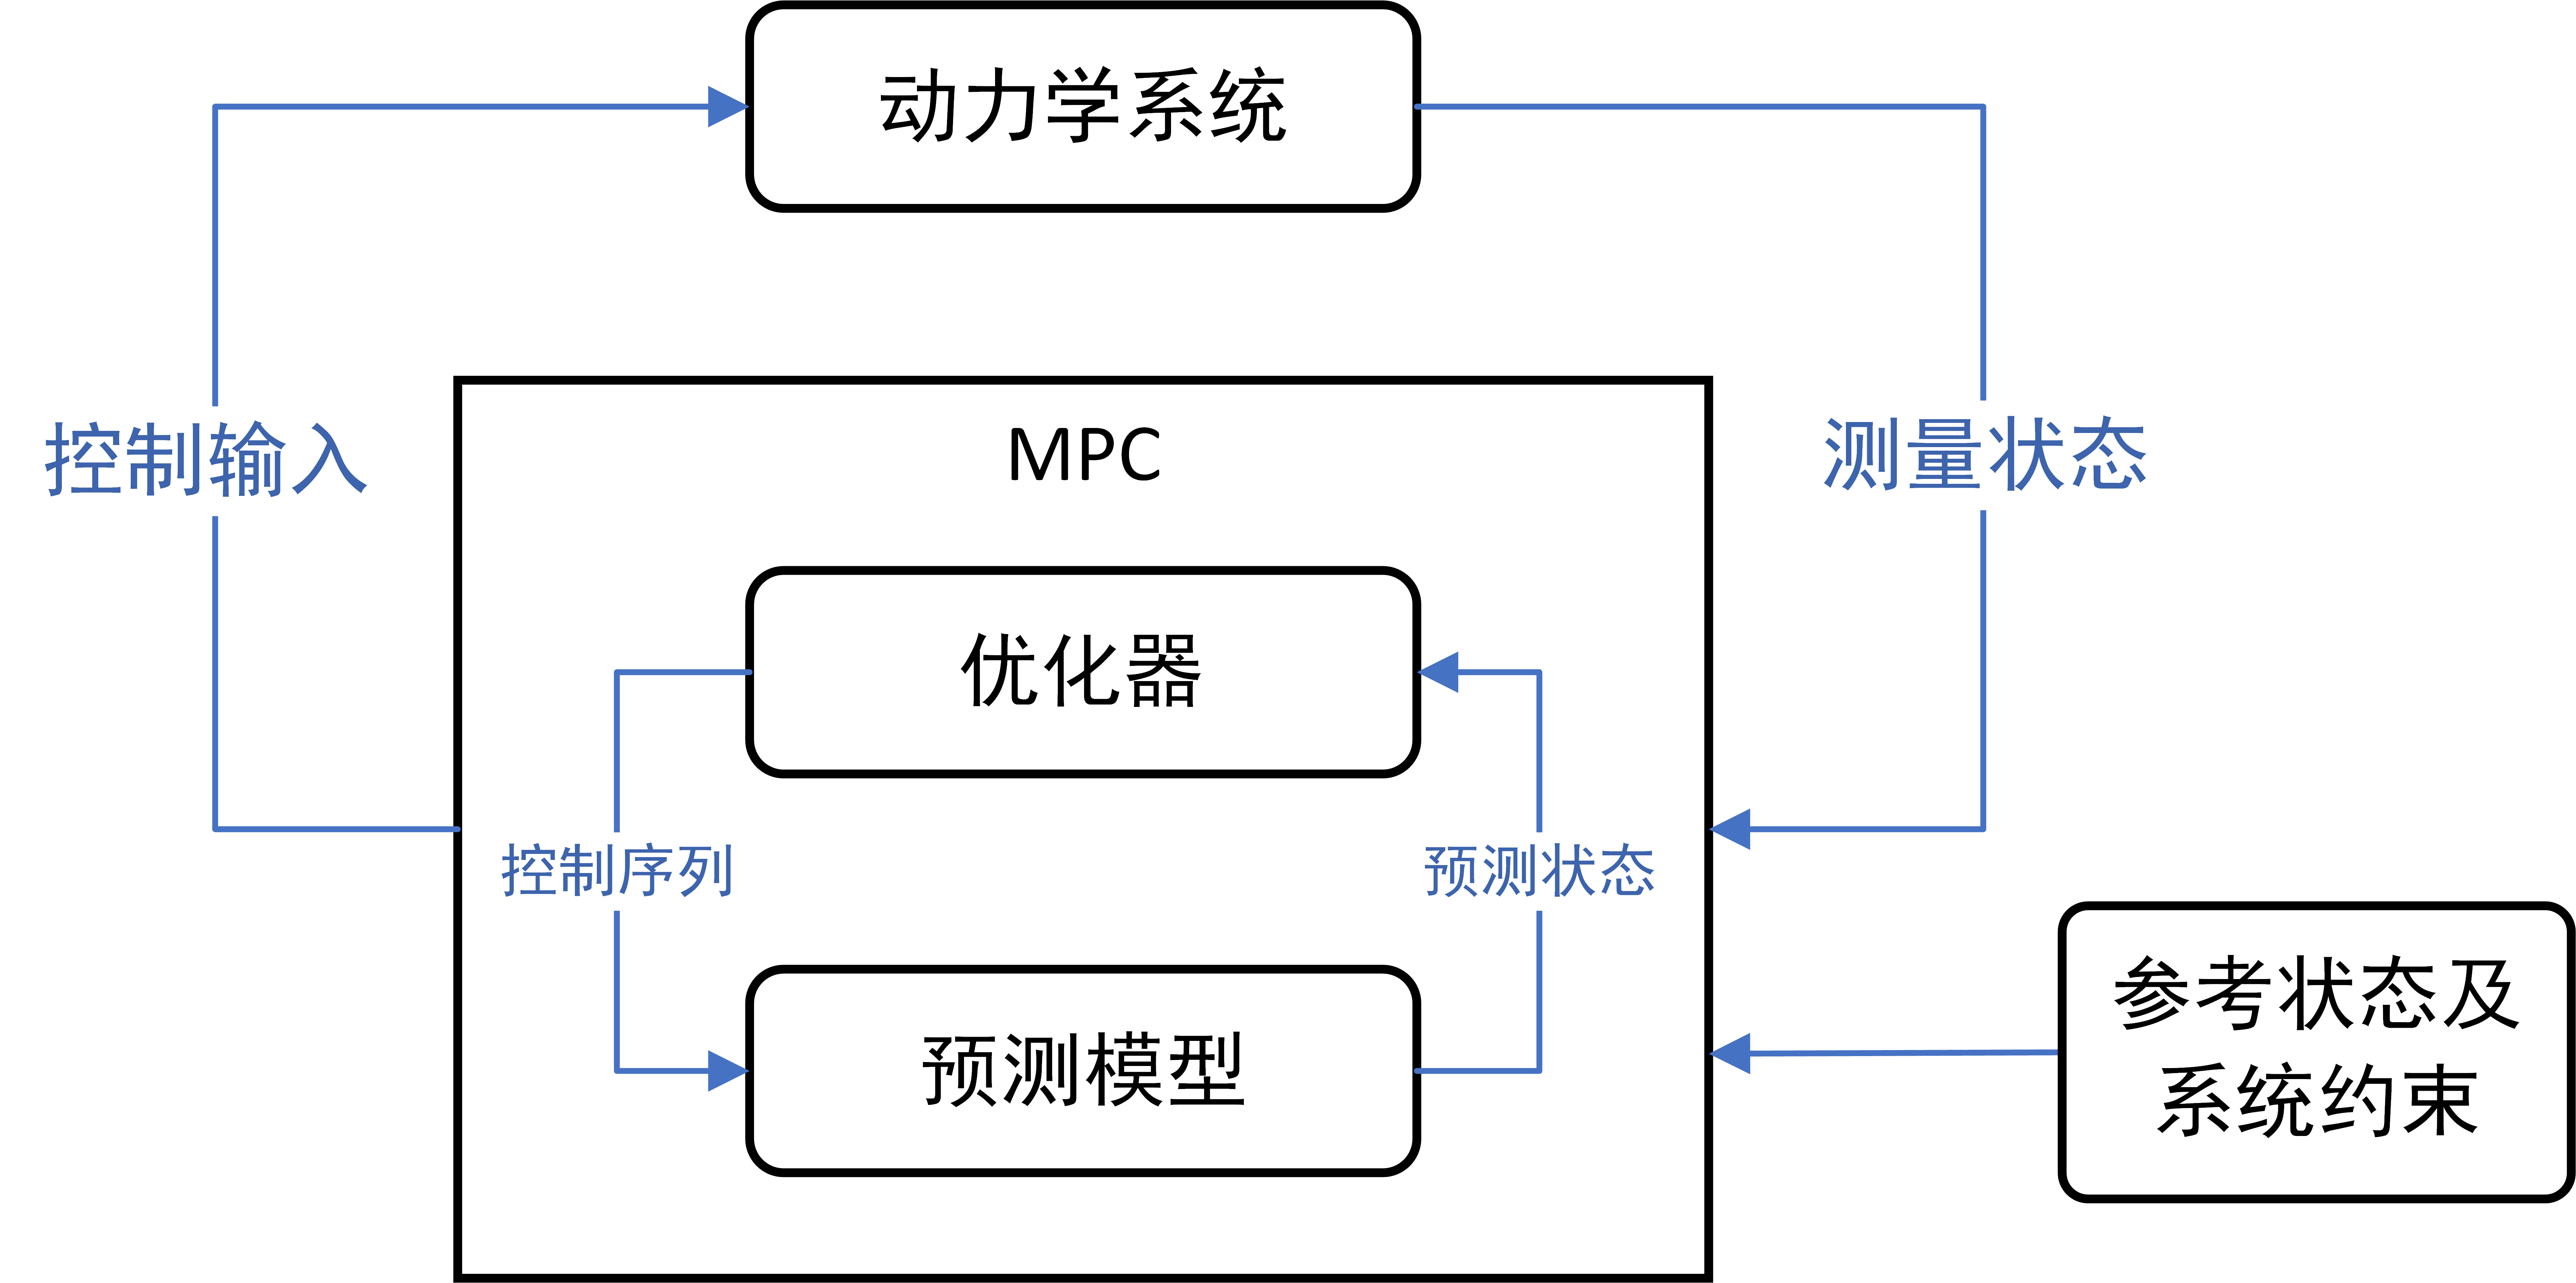
\includegraphics[width=0.8\linewidth]{images/chapter4/MPC控制闭环图.png}
    \caption{MPC控制回路}
    \label{f.MPC_control_loop}
\end{figure}

MPC主要包含两个部分,预测模型和优化器,MPC的控制回路如图\ref{f.MPC_control_loop}所示。在MPC控制回路中,它从动态系统中接收参考状态、系统约束和测量状态,并将控制输入输反馈回动力学系统。MPC根据预测模型在一定范围内的控制输入序列计算预测输出,而优化器解决二次规划( QP )问题:

\begin{equation}
\begin{aligned}
 & \min_{U,X}\int_{t=0}^T 
 \begin{Vmatrix}
     h(x(t),u(t))-y_{ref}
 \end{Vmatrix}_Q^2dt +
  \begin{Vmatrix}
     h(x(T))-y_{N,ref}
 \end{Vmatrix}_{Q_N}^2
 \\
& \text{subject to} \quad \dot{x}=f(x(t),u(t)); \\
& u(t) \in \mathbb{U} \\
& x(t) \in \mathbb{X} \\
& x(0) = x(t_0)
\end{aligned}
\end{equation}

其中$u(t)$和$x(t)$分别表示$t$时刻的控制输入和系统状态;$T$是预测范围,代表向前预测的时间步数;$y_{ref}$和$y_{N,ref}$分别为预测时域和终终点参考状态中的阶段参考状态;$Q$和$Q_N$是阶段状态和终点状态的权重矩阵;$F(\cdot )$和$h(\cdot )$分别为预测模型和系统输出函数;$\mathbb{U}$和$\mathbb{X}$是控制输入和系统状态的约束。

要调整 MPC,需要遵循几个重要步骤。首先,选择控制范围$T$,考虑权衡控制性能和计算负担。为了找到一个平衡这些因素的最优值,水平在模拟过程中逐步增加,并在评估改善控制性能的同时保持 MPC 的实时运行。此外,MPC 允许通过将矩阵$\symbf{Q}$中的权重因子分配给每个目标来确定多个控制目标的优先级。在这个特殊的工作中,偏航角$\psi $被赋予了最高的优先级,其次是位置状态$x, y, z$。终端成本与在预测范围的末端的系统的最终状态有关。终端状态$Q_N$处的加权矩阵反映了达到期望的稳态或目标的相对意义。权重越高,表示越强调达到所需的终端状态。本工作中为保证控制器稳定性,$Q_N$被设置为等于 $\symbf{Q}$ 中的值,以提供较少的激进控制。

\section{轨迹跟踪仿真验证}

通过前文所述内容,本文已搭建起BlueROV2的动力学模型,通过最小二乘法和扩展卡尔曼滤波器辨识出两组水动力参数,为了比较两个算法在动力学模型辨识上的优劣,本文通过设计不同的轨迹跟踪任务以测试两组系数在实际工作中的表现。

\subsection{仿真参数设置}

本章节根据表\ref{t.physical_params}设置BlueROV2的物理参数,通过URDF文件定义BlueROV2模型并导入UUV Simulator中。表\ref{t.MPC_params}列出了MPC相关参数,预测视界为60,采样时间为0.05s,系统向前推测3s。

\begin{table}[htb]
  \centering
  \caption{MPC控制参数表}
  \zihao{5}
  \label{t.MPC_params}
  \begin{tabular}{cl}
  \hline
参数名 & 参数值\\
\hline
预测视界 & 60s \\
采样间隔 & 0.05s \\
$Q$      & [350, 350, 350, 10, 10, 150, 10, 10, 10, 10, 10, 10, 15, 15, 15, 0.5] \\
$Q_N$   & [350, 350, 350, 10, 10, 150, 10, 10, 10, 10, 10, 10]  \\
OCP时间 & 7ms \\
\hline
\end{tabular}
\end{table}

\subsection{圆形轨迹跟踪仿真验证}

本章节设置圆形曲线作为参考轨迹,使BlueROV2从初始位置$[0,0,-0.5]\text{m}$处出发,沿参考轨迹做绕行运动,定义圆形曲线方程为:
\begin{equation}
    [x_r, y_r, z_r]^T = \left\{\begin{matrix}
  -R\cos(\frac{tv}{R}) + x_0 \\
  -R\sin(\frac{tv}{R}) + y_0 \\
  z_0 
\end{matrix}\right.
\end{equation}
定义绕行偏航角方程为:
\begin{equation}
    \psi_r = \frac{tv}{R}-0.5\pi
\end{equation}
其中,$x_r,y_r, z_r,\psi_r$为参考点的坐标值和参考点处的参考偏航角,$R$为圆形半径,$x_0,y_0,z_0$为初始位置坐标,$v$为期望绕行速度,曲线设置满足$x_0=y_0=0$,$z_0=-20\text{m}$,$R=2\text{m}$,$v=1.5\text{m/s}$。

将扩展卡尔曼滤波器辨识出的水动力参数代入轨道追踪控制框架,在其轨迹收敛后,得到其轨迹跟踪曲线与位置跟踪误差分别如图\ref{f.circle_track_traj}和图\ref{f.circle_track_error}所示。

\begin{figure}[hbt]
    \centering
    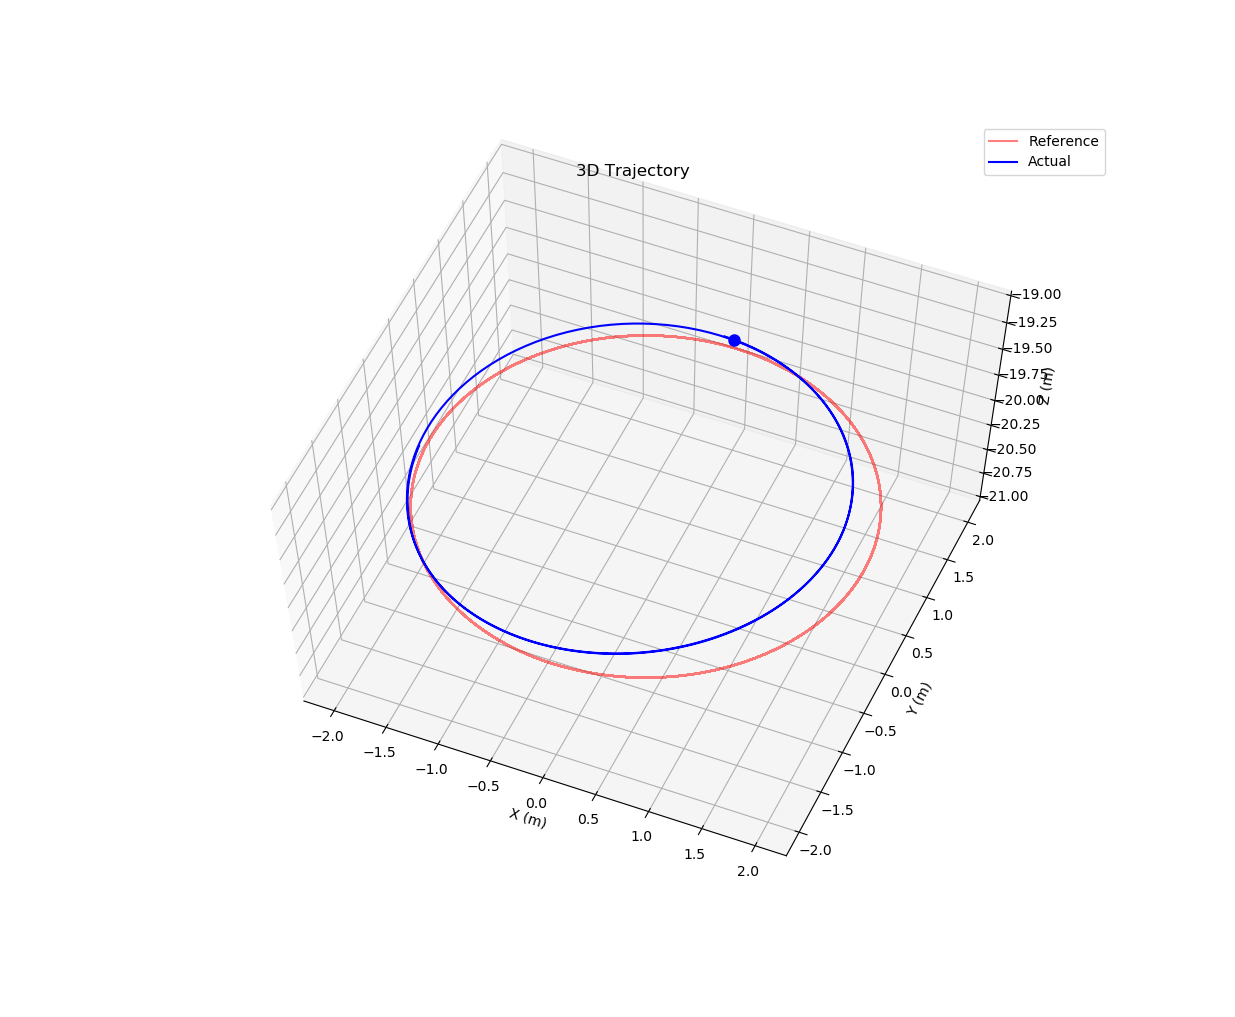
\includegraphics[width=0.8\linewidth]{images/chapter4/circle_track_traj.png}
    \caption{EKF辨识系数下圆形轨迹跟踪曲线}
    \label{f.circle_track_traj}
\end{figure}
\begin{figure}[hbt]
    \centering
    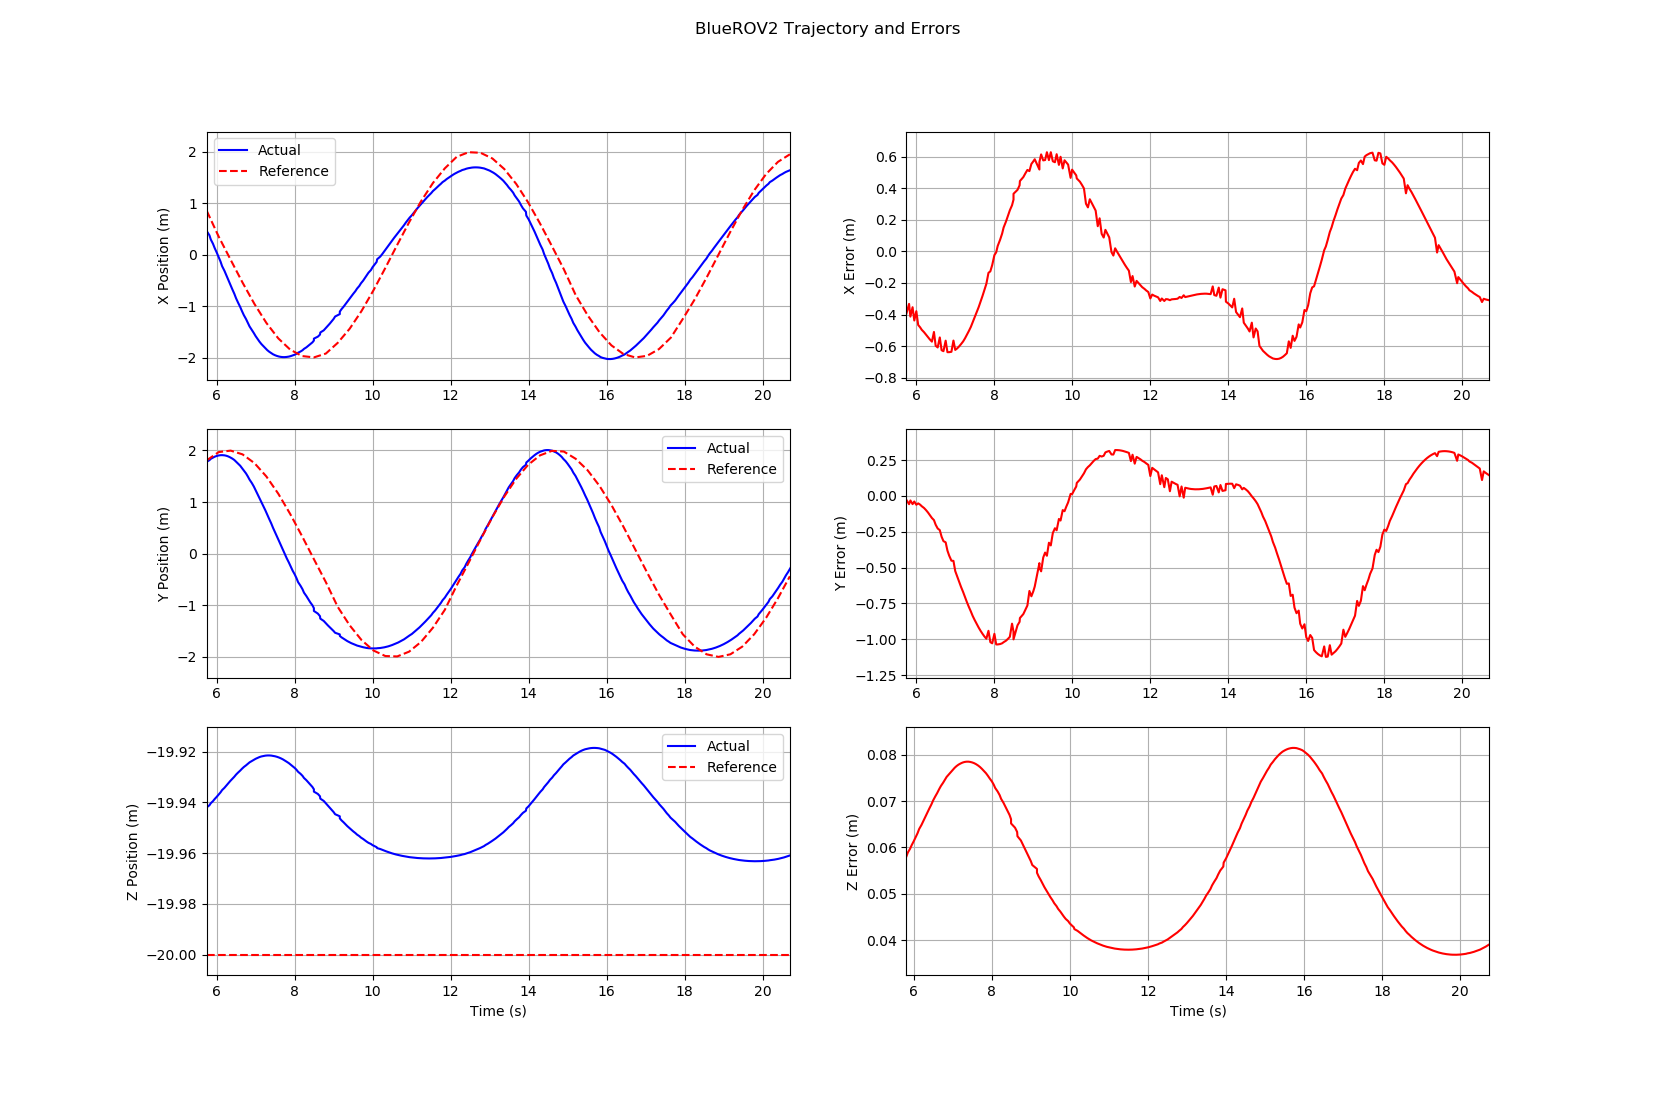
\includegraphics[width=0.8\linewidth]{images/chapter4/circle_traj_error.png}
    \caption{EKF辨识系数下圆形轨迹跟踪误差}
    \label{f.circle_track_error}
\end{figure}

将最小二乘算法辨识出的水动力参数代入轨道追踪控制框架,在其轨迹收敛后,得到其轨迹跟踪曲线与位置跟踪误差分别如图\ref{f.ls_circle_track_traj}和图\ref{f.ls_circle_track_error}所示。

\begin{figure}[hbt]
    \centering
    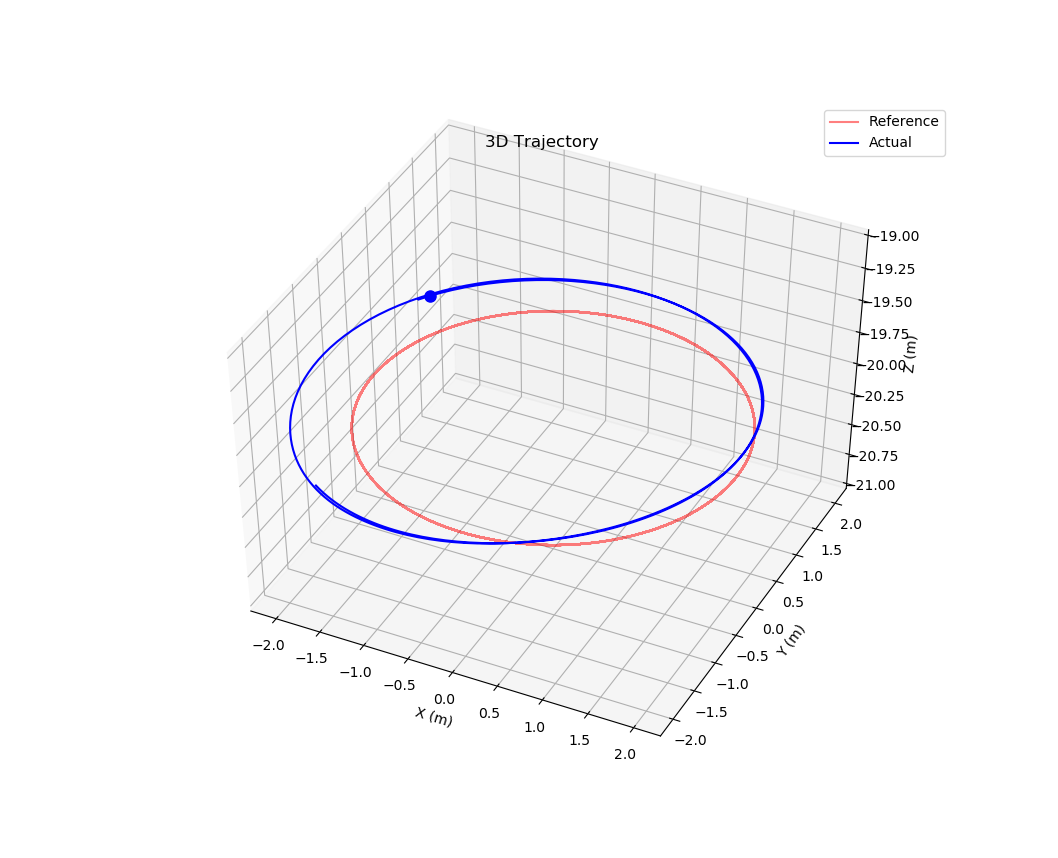
\includegraphics[width=0.8\linewidth]{images/chapter4/ls_circle_traj.png}
    \caption{最小二乘辨识系数下圆形轨迹跟踪曲线}
    \label{f.ls_circle_track_traj}
\end{figure}
\begin{figure}[hbt]
    \centering
    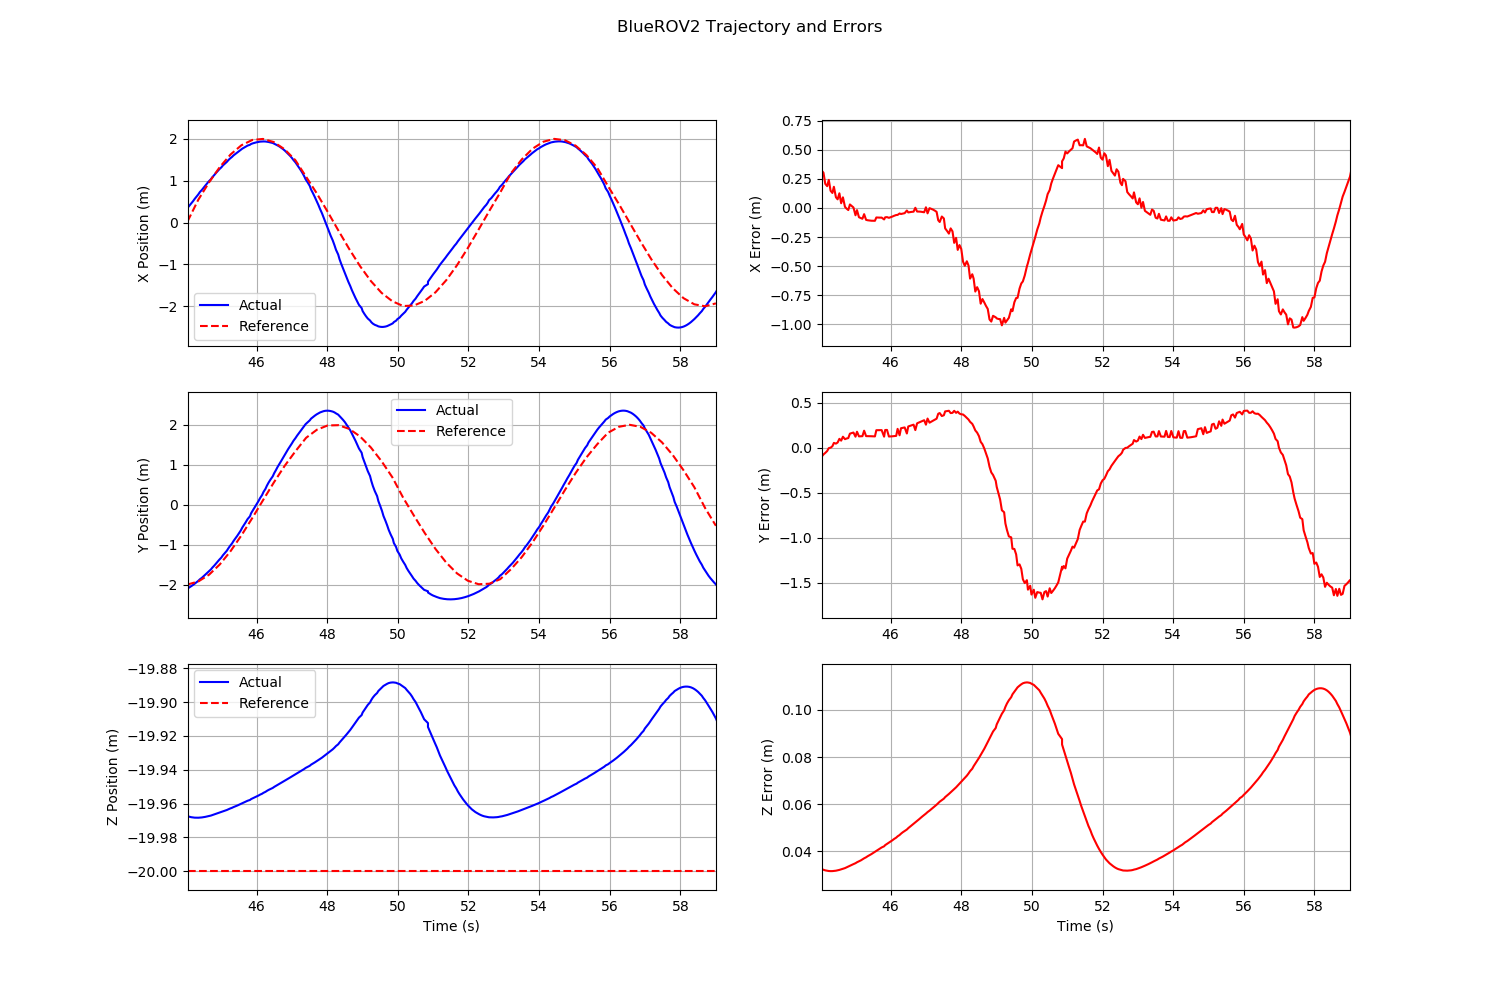
\includegraphics[width=0.8\linewidth]{images/chapter4/ls_circle_error.png}
    \caption{最小二乘辨识系数下圆形轨迹跟踪误差}
    \label{f.ls_circle_track_error}
\end{figure}

通过对比可以看出,最小二乘辨识系数下的圆形轨迹跟踪相较于参考点的超调量大,最大误差占位置变化曲线峰值的25\%,而EKF辨识系数下的圆形轨迹跟踪能更准确地拟合参考轨迹,其在$x$方向上的轨迹跟踪误差依然达到25\%的占比,但是在$Y$方向上的轨迹跟踪误差仅达12\%,同时,两个辨识方法辨识出的系数在$z$方向上的深度控制均有较好的表现。

\subsection{双纽线轨迹跟踪仿真验证}

本章节设置双纽线为参考轨迹,使BlueROV2从初始位置$[0,0,-0.5]\text{m}$处出发,沿参考轨迹做绕行运动,定义双纽线方程为:

\begin{equation}
    [x_r,y_r,z_r]^T=\left\{\begin{matrix}
        A\cos(ft)+x_0 \\
        A\sin(ft)\cos(ft)+y_0 \\
        z_0
    \end{matrix}\right.
\end{equation}
其中,$A$为双纽线长轴距离,$f$为环绕频率,曲线设置满足$A=2m$,$f=0.5s^{-1}$,采样频率为20Hz。

将扩展卡尔曼滤波器辨识出的水动力参数代入轨迹追踪控制框架,在其轨迹收敛后,得到其轨迹跟踪曲线与位置跟踪误差分别如图所示。

\begin{figure}[hbt]
    \centering
    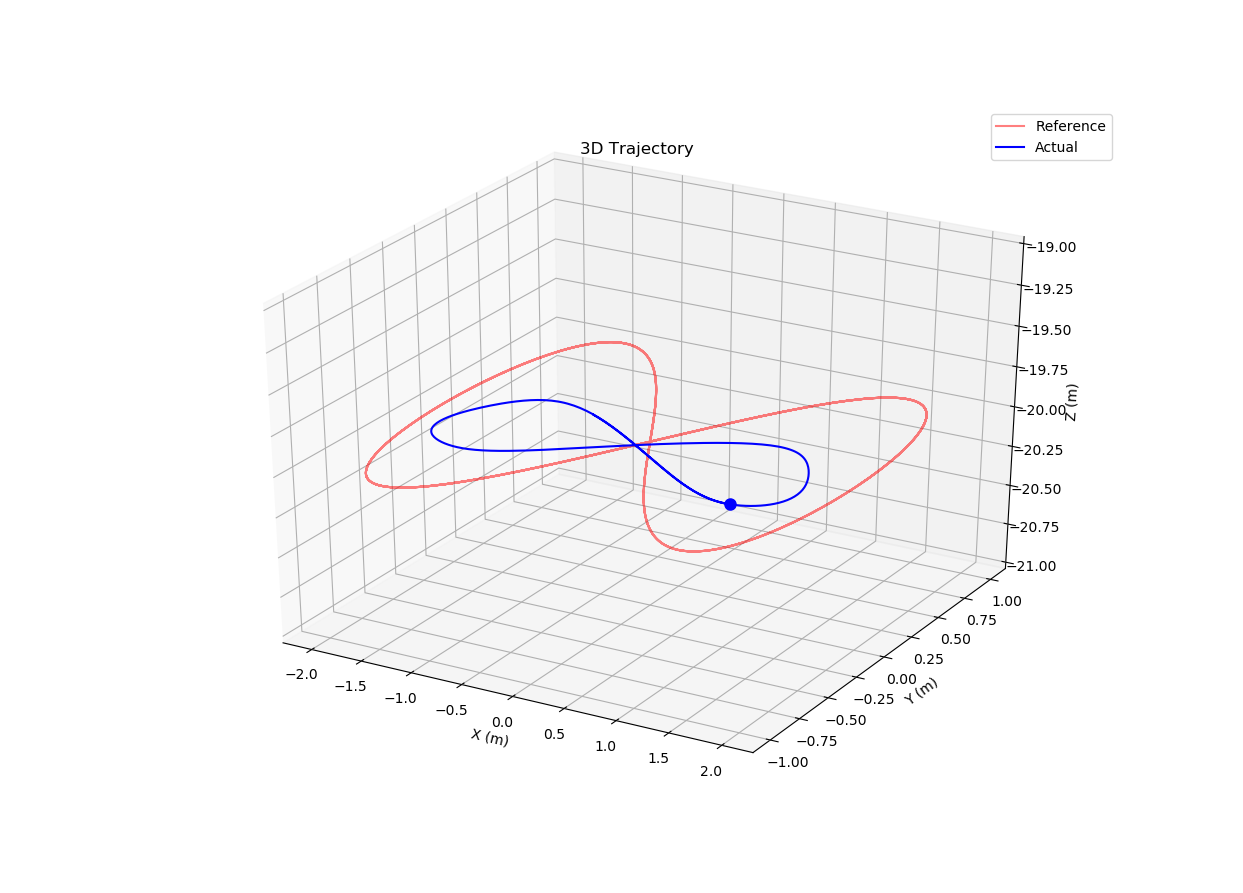
\includegraphics[width=0.8\linewidth]{images/chapter4/lem_traj.png}
    \caption{EKF辨识系数下双纽线轨迹跟踪曲线}
    \label{f.lem_track_traj}
\end{figure}
\begin{figure}[hbt]
    \centering
    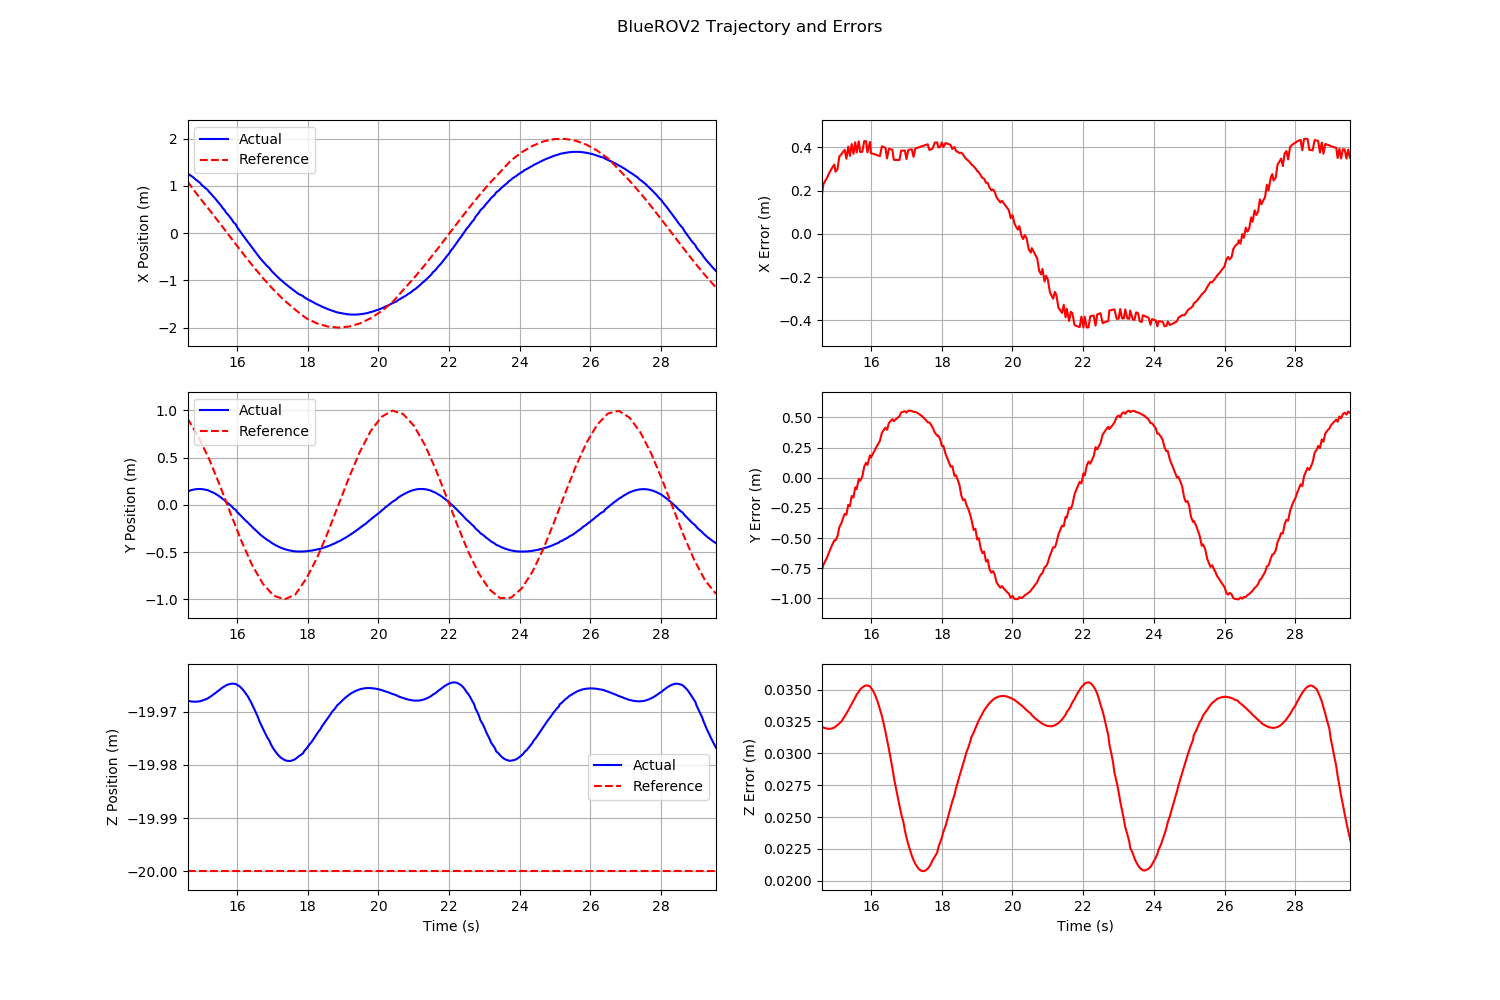
\includegraphics[width=0.8\linewidth]{images/chapter4/lem_error.png}
    \caption{EKF辨识系数下双纽线轨迹跟踪误差}
    \label{f.lem_track_error}
\end{figure}

将最小二乘算法辨识出的水动力参数代入轨迹追踪控制框架,在其轨迹收敛后,得到其轨迹跟踪曲线与位置跟踪误差分别如图\ref{f.lem_track_traj}和图\ref{f.lem_track_error}所示。

\begin{figure}[hbt]
    \centering
    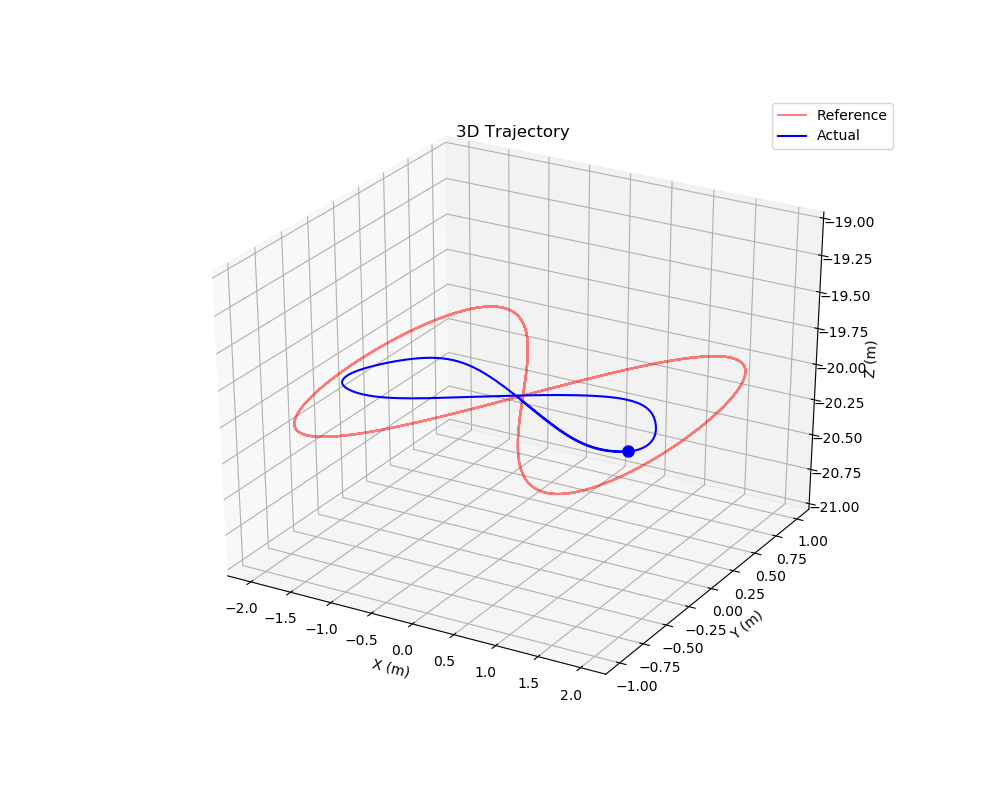
\includegraphics[width=0.8\linewidth]{images/chapter4/ls_lem_traj.png}
    \caption{最小二乘辨识系数下双纽线轨迹跟踪曲线}
    \label{f.lem_track_traj}
\end{figure}
\begin{figure}[hbt]
    \centering
    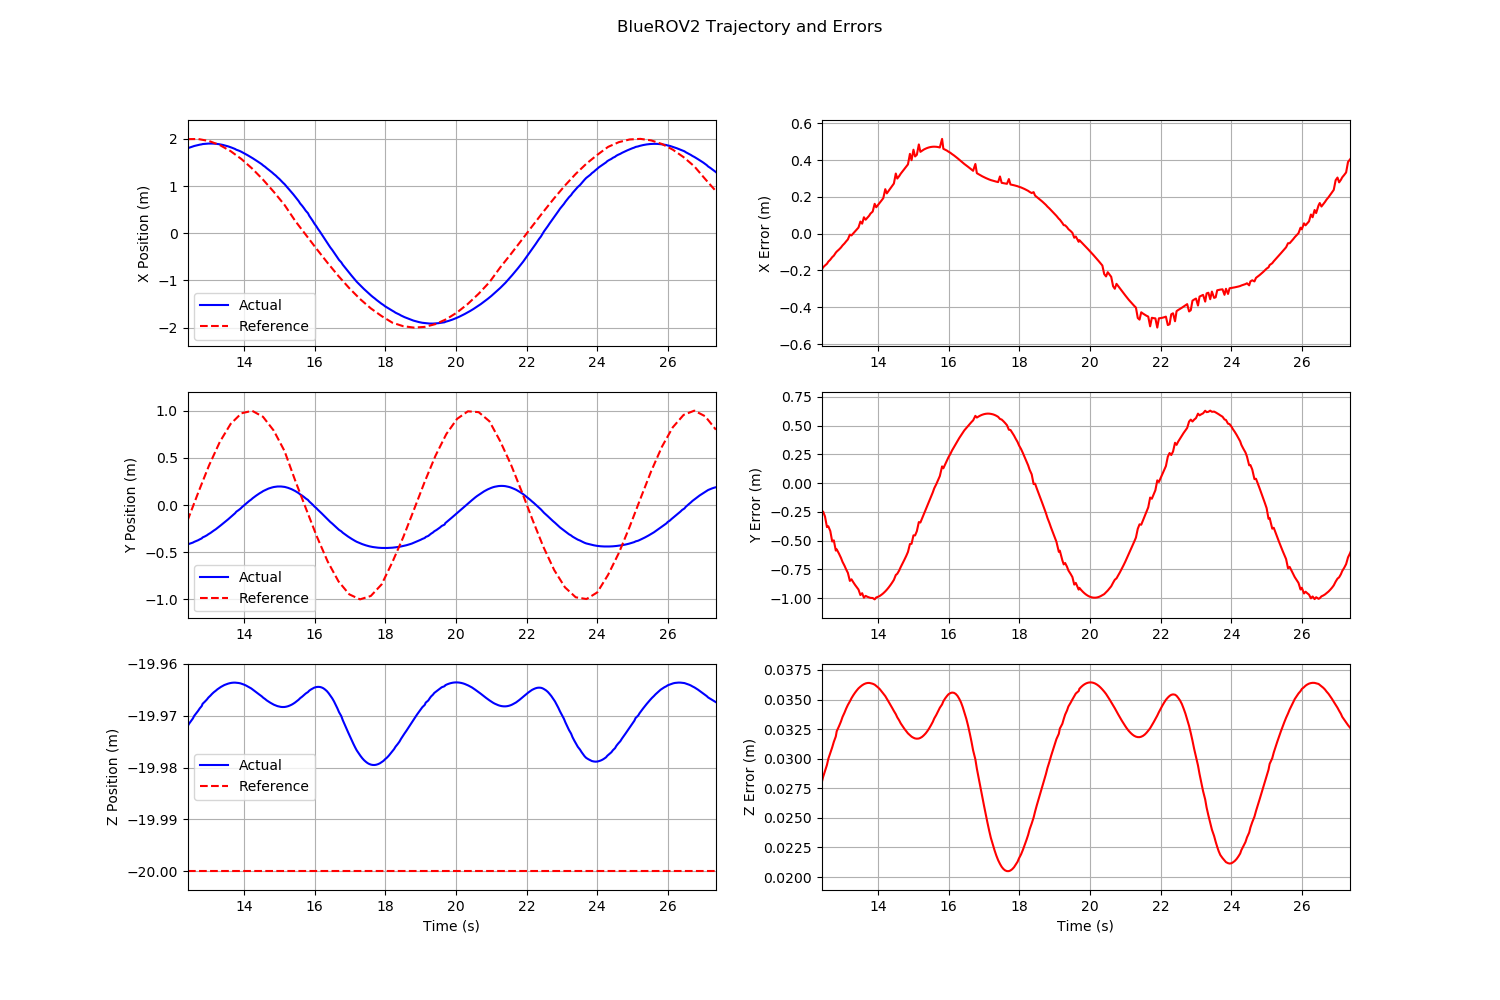
\includegraphics[width=0.8\linewidth]{images/chapter4/ls_lem_error.png}
    \caption{最小二乘辨识系数下双纽线轨迹跟踪误差}
    \label{f.lem_track_error}
\end{figure}

通过对比可以看出,最小二乘和EKF辨识出的系数,在双纽线轨迹跟踪上的表现均不如圆形轨迹跟踪,且尤其在$y$轴方向上误差较大,而在$z$轴方向上均能保持较好的深度控制。此外,在$x$轴方向上,二者最大误差均达到0.4,占参考轨迹最大峰值的25\%,可以认为两者在更为复杂情况下的轨迹跟踪上较无显著差别。

\section{本章小结}

本章节在前一章节辨识水动力参数的基础上,通过UUV Simulator仿真平台,实现了MPC控制器,设计BlueROV2的轨迹跟踪任务。分别设计了圆形和双纽线形两种参考轨迹,再分别代入由最小二乘系数辨识和由扩展卡尔曼滤波器辨识出的水动力参数,分析其轨迹跟踪曲线及误差表现,发现在参考轨迹为圆形时,基于扩展卡尔曼滤波器的轨迹跟踪误差较小,表现良好;而两组水动力系数在双纽线形更为复杂的情况下轨迹跟踪表现并无显著差异。

\newpage



